%%%%%%%%%%%%%%%%%%%%%%%%%%%%%%%%%%%%%%%%%%%
%%% DOCUMENT PREAMBLE %%%
\documentclass[12pt]{report}
\usepackage[english]{babel}
%\usepackage{natbib}
\usepackage{url}
\usepackage[utf8x]{inputenc}
\usepackage{amsmath}
\usepackage{graphicx}
\graphicspath{{images/}}
\usepackage{parskip}
\usepackage{fancyhdr}
\usepackage{vmargin}
\usepackage[T1]{fontenc} % Use 8-bit encoding that has 256 glyphs
\usepackage{booktabs} % for nice lines in tables
\setmarginsrb{3 cm}{2.5 cm}{3 cm}{2.5 cm}{1 cm}{1.5 cm}{1 cm}{1.5 cm}

\title{Applying Reinforcement Learning to Bomberman}								
% Title
\author{Hein-Erik Schnell, Karl Thyssen}						
% Author
\date{\today}
% Date

\makeatletter
\let\thetitle\@title
\let\theauthor\@author
\let\thedate\@date
\makeatother

\pagestyle{fancy}
\fancyhf{}
\rhead{\theauthor}
\lhead{\thetitle}
\cfoot{\thepage}

% displays code within text
\newcommand{\code}[1]{{\fontfamily{pcr}\selectfont #1}}
\newcommand{\state}[1]{$\left\lbrace #1 \right\rbrace$}
%%%%%%%%%%%%%%%%%%%%%%%%%%%%%%%%%%%%%%%%%%%%
\begin{document}

%%%%%%%%%%%%%%%%%%%%%%%%%%%%%%%%%%%%%%%%%%%%%%%%%%%%%%%%%%%%%%%%%%%%%%%%%%%%%%%%%%%%%%%%%

\begin{titlepage}
	\centering
    \vspace*{0.5 cm}
    
\includegraphics[scale = 0.075]{uni_hd_logo.jpg}\\[1.0 cm]	% University Logo
\begin{center}    \textsc{\Large   Fundamentals of Machine Learning}\\[2.0 cm]	\end{center}% University Name
	\textsc{\Large Final Project  }\\[0.5 cm]				% Course Code
	\rule{\linewidth}{0.2 mm} \\[0.4 cm]
	{ \huge \bfseries \thetitle}\\
	\rule{\linewidth}{0.2 mm} \\[1.5 cm]
	
	\begin{minipage}{0.4\textwidth}
		\begin{flushleft} \large
		%	\emph{Submitted To:}\\
		%	Name\\
          % Affiliation\\
           %contact info\\
			\end{flushleft}
			\end{minipage}~
			\begin{minipage}{0.4\textwidth}
            
			\begin{flushright} \large
			\emph{Submitted By :} \\
			Hein-Erik Schnell\\
			Karl Thyssen  
		\end{flushright}
           
	\end{minipage}\\[2 cm]
	
	%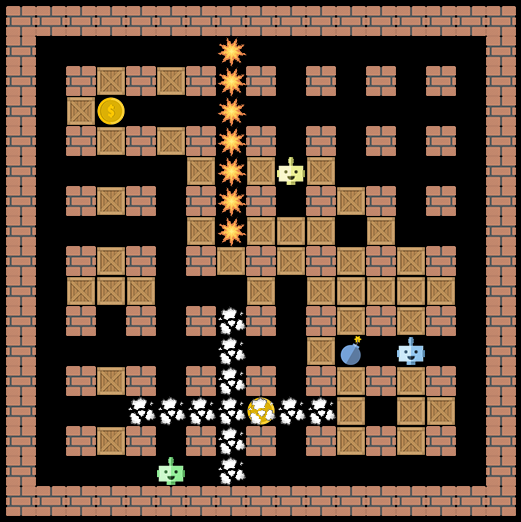
\includegraphics[scale = 0.3]{Bomberman_title.png}
    
    
    
    
	
\end{titlepage}

%%%%%%%%%%%%%%%%%%%%%%%%%%%%%%%%%%%%%%%%%%%%%%%%%%%%%%%%%%%%%%%%%%%%%%%%%%%%%%%%%%%%%%%%%

\tableofcontents
\pagebreak

%%%%%%%%%%%%%%%%%%%%%%%%%%%%%%%%%%%%%%%%%%%%%%%%%%%%%%%%%%%%%%%%%%%%%%%%%%%%%%%%%%%%%%%%%
\renewcommand{\thesection}{\arabic{section}}
\chapter{Preliminaries}
\section{Heins thoughts}
Tasks to be done are:
	\begin{itemize}
		\item Find a suitable \textit{state representation} to be then passed to an estimator to estimate the expected reward for each of the possible actions
		\item Find a suitable rewards in order to communicate the goals of the game to the agent
		\item Find a suitable model which estimates the expected reward for each possible action at the current state of the game.
	\end{itemize}

\subsection{State representation}
My proposal is a 2D numpy array. Each row (first index) represents a single state. Each column represents a feature. All available information is stored within each agent in the dictionary \code{self.game\_state}. What features do we store?
	\begin{itemize}
		\item For each cell:
		\begin{itemize}
			\item \textbf{Crate, wall, free \state{1,-1,0}}: The same representation is provided by \code{self.game\_state}. Only it has to be reshaped into a 1D-array. 
			\item \textbf{Cell contains agent \state{0,1}}
			\item \textbf{Cell contains opponent \state{0,1}}: This and the point above need to be stored seperately because it is possible for agent and opponent to occupy the same cell. It would just be impossible to distinguish whether a cell is occupied by just one or more opponents. But this should be a negligible issue. 
			\item \textbf{Cell contains coin \state{0,1}}
			\item \textbf{Explosion on cell}: Provided as 2D-numpy array by \code{self.game\_state}.
			\item \textbf{Danger level \state{0,\dots,4}}: How many time steps until an explosion will hit the cell.
		\end{itemize}
		\item Just once at the end of the array:
		\begin{itemize}
			\item \textbf{Current step number \state{1,\dots,400}}
			\item \textbf{Bomb action possible \state{0,1}}
			\item \textbf{Danger level:} This is a danger level for the agent. It is not necessary but provides a clearer measure of whether the agent is actually in danger. I propose to calculate this by multiplicating the danger level of each cell with the \textit{Cell contains agent} entry of each cell and then take the maximum of all the results. This way we will only get a non-zero value if the agent is on a cell with a danger level $>0$.
			\item \textbf{Reward already received in this episode}
			\item \textbf{Reward received at the end of the episode}: This one has to be added subsequently at the end of the episode to each ocurred state.
			\item \textbf{Reward gained after this state occurred:} This one is the difference of the two above. This should be our \textit{target} which we aim to maximize.
			\item \textbf{Agent touches opponent \state{0,1}}: The simple agents consider dropping a bomb if they touch an opponent. This may be a very good indicator for dropping a bomb for our model.
		\end{itemize}
	\end{itemize}
This gives us $6$ entries for each cell and $7$ entries at the end of the array. There are $17\times17$ cells in the arena. However, the cells located at the rim are always \textit{walls}. These do not need to be stored. What remains is a $15\times15$ grid. I am not sure whether we want to store cells with \textit{walls} at all, because these are always the same. They should add nothing to the state of the game.\\
Therefore we have $15\times15=225$ entries ($15\times15-7\times7=176$ if we don't store walls) plus $7$ at the end of the array for each state (time step). Storing these total $232$($183$) entries in a numpy array might produce big amounts of data. We should consider specifying the data type explicitly. However, the numpy documentation states that the data type is chosen as the minimum type required to hold the objects in the sequence.

\subsection{Rewards}
The most rewarded actions should be those which will win us the game. Those are collecting coins (1 point) and killing opponents (5 points). Therefore, I propose the same scaling between those two when rewarding them. \\
Subgoals which we consider helpful for winning should be rewarded too, but only with few points. It should be almost impossible to substitute the \textit{winning actions} (coins and killing) with \textit{helpful actions} (destroying crates). \\
I also propose a penalty of $-1$ for every action so that the agent learns to act as efficiently as possible. \\
Dying should be (beware! wordplay:) gravely punished. 
\begin{figure}[h]
	\centering
	\begin{tabular}{c|c}
		Action & Reward\\
		\toprule
		Collect coin & 100\\
		Kill opponent & 500\\
		Destroy crate & 1-2 per crate\\
		Perform action & -1\\
		Die & -500fd
	\end{tabular}
\end{figure}

\subsection{Estimator} 
I don't know much about neural networks which is why I spent most of my thoughts on how to implement this with the models we used in the exercises. Plus, I like the idea of the challenge to come up with an agent which doesn't use a neural network. \\
Since we want to estimate the expected reward of performing an action at in a given state, we need a regressor. This regressor needs to be highly flexible in order to cope with the variety of states. I guess the most flexible regressor we used would be a \textit{Random Forest Regressor}. On the one hand, this one would need tons of learning data but on the other hand, which proper regressor doesn't?\\
This means, we would plug the data of the states and the received rewards into the model and get an estimate of what reward we could expect for what action. Since we need to distinguish between the six possible actions, we need six Random Forests. One for each action. Each forest trained only with the states after which the respective action was performed. This also means that we need to store all data in six different set for six possible actions or store the action performed afterwards in the \textit{state vector}.

\subsection{Learning algorithm}
I propose to use the Max-Boltzmann (MB) method as described in \cite{paper} or something similar. It is mostly a $\epsilon$-greedy algorithm. But when it decides to explore, it doesn't choose randomly among the remaining actions but assigns probabilities corresponding to the value (expected reward) of the remaining action. This way, exploration is not just random but more targeted.\par

There is no point in letting the agent learn after every single episode. In the long run those learning interruptions will cost us a lot of time. Plus, it is very unlikely that the next episodes are similar to the one before which means that the learning will most likely not be applied in the subsequent episodes. Thus, the learning process itself should be divided into learning intervals of many episodes, say 100 to 1000, maybe even 10000 episodes, given the number of possible states. While we're already using the term \textit{episodes}, let's call those learning intervals \textit{seasons}.\par
I propose the following procedure:
\begin{enumerate}
	\item Use the provided simple agent as our agent to play the first season. I would use the MB algorithm already in the first episode. This already gives us the possibility of exploration which I consider as important since the simple agent is fully determined and hard coded.
	\item Use the data of the first season to train our model. 
	\item From now on, let the agent rely only on the predictions of our model. Create data, explore according to the MB algorithm. 
	\item Use the data of all former seasons to again train our model.
	\item Repeat the two former steps.
\end{enumerate}
The simple agents should be good sparring partners to start with. They are very good at avoiding bombs but sometimes lack the ability to collect coins. We might improve this ability in the simple agent code to get better starting conditions. Maybe by automatically decreasing the distance (and thus increasing importance) of coins.
\subsection{Necessary functions}
Some functions that need to be implemented in order to prepare everything:
\begin{itemize}
	\item Calculate danger levels of each cell
	\item Insert \textit{coins} into \textit{state vector}
	\item Insert \textit{opponents} into \textit{state vector}
	\item Insert \textit{self} into \textit{state vector}
\end{itemize}
We need to decide what structure the \textit{state vector} should have. There are two ways:
\begin{enumerate}
	\item All features of a concerning cell (coin, opponent, self, danger level,...) subsequently. The all features of the next cell and so on \dots
	\item All data of one feature (e.g. coin) for all cells, then all data of the next feature for all cells and so on \dots
\end{enumerate}
In both cases, the functions that insert the values into the array should make use of the slicing possibilities of numpy arrays (e.g. \code{x[starting point:end point:stepsize]}). In the first case, only every sixth entry represents the same feature. In the second case, the first hundred entries represent only one feature for different cells.

\section{Karls thoughts}

How this project can be approached:
	\begin{itemize}
		\item Neural Network approach \textit{vs.} Classical Machine learning approach
		\begin{itemize}
			\item Supervised learning \textit{vs.} Reinforcement learning \textit{vs.} Unsupervised learning
			\item Feature selection to determine relevant information the agent should "see" and learn from
		\end{itemize}
		\item Data management for training - not necessary as we will be collecting all the relevant data while training rather than using a large pre-compiled dataset
	\end{itemize}

As we do not have access to more than our own laptops which can not be classed as high performance systems with low end dedicated GPUs training neural networks may be impractical and time consuming.

\subsection{Neural Networks}
As we didn't cover neural networks in the lecture but are allowed to apply them to this Project I explored it as an option despite knowing we are likely to select the classical approach.
Some algorithms that are worth exploring are:
	\begin{itemize}
		\item Supervised learning:
		\begin{itemize}
			\item Gradient descent involves forming a continuous error function using rewards to minimize
		\end{itemize}
		\item Reinforcement learning:
		\begin{itemize}
			\item Q-Learning (as covered in lectures)
			\item Genetic Algorithm:
			\begin{itemize}
				\item Training occurs through improvements from generation to generation by improving the strength and bias values for the edges of the neural network (stored in a 1D array). Each generation has a set number of instances that follow a variation of the previous generations values. To decide which of the instances in the previous generation had the best strength and bias values a scoring system must be created based on the performance of each instance.
				\item Outputs are predetermined as 5 movement options (up, down, left, right, stand still) and the Bomb placement option
				\item Factors to be decided on:
				\begin{itemize}
					\item Inputs e.g. \textit{weighted score of distance to enemies/crates/coins/bombs}
					\item Number of hidden layers and nodes (not sure how this is done yet)
					\item Method for genetic variation e.g. \textit{ranking by score and weighting the likelihood for this process to be selected, random selection}. This is the exploitation aspect. Some values however should be randomly changed or multiple arrays crossed together (like nature) to increase the likelihood of finding the global minimum rather than local (exploration.
				\end{itemize}
			\end{itemize}
		\end{itemize}
	\end{itemize}		

\subsection{Classical approach}
We could use Q-learning to train a $\epsilon$-greedy agent. We want to find the optimal policy \textbf{Q} to solve the game.

Here its important to identify the 2 sets of attributes that contribute to decision making, \textbf{state} and \textbf{action}. The state will be input to decision making function to determine the action, the features that describe the state however must first be decided on.
To reduce runtime it may be advantageous to perform a dimension reduction if it becomes clear that some features for example the states of the cells outside of a 5x5 radius around the agent have very little impact on the decision. This could be particularly important in the early tests before the final train to reduce training time required when for example testing various reward value boundaries.

\subsubsection{State appraisal}
Before a decision can be reached as to the next action clearly the state of the board must first be assessed. With an almost infinite number of possible inputs possible it is important to have as few and as relevant features as possible.

Ideas to test/discuss:
\begin{itemize}
	\item Are all accessible fields relevant
	\item Is it possible to approximate the state with knowledge about only the non-empty fields. In extreme cases this can be 2 (final 2 agents) or 176 (all fields occupied, although this is a stalemate) so this is likely not constructive.
	\item How should the distances to other agents or items be stored? Possibilities include:
	\begin{itemize}
	\item The route that could be taken
	\item Only the coordinates
	\item The number of moves required to move the the desired opponent or coins field and the direction. Here the shorter route could also be through boxes and therefore include bomb wait times
	\end{itemize}	 
	\item Should any previous states have a weighted input? - probably not, could be useful in some edge cases maybe?
\end{itemize}

\subsubsection{Rewards}
Naively we want to positively reinforce proactive, safe actions and negatively reinforce hazardous or even fatal actions so we should set our rewards based on this structure. This may however not always lead to the optimal solution as there are some situations where a sacrifice can lead to a greater boon in later steps e.g. \textit{queen sacrifice for checkmate in chess}.

We have essentially 3 choices for how to issue rewards:
\begin{itemize}
	\item Updating Q after each episode:
	\begin{itemize}
		\item This leads to faster training times as the entire episode can play out without interruptions, however each episode leads to slower improvement as the Agent can only perceive the results of all decisions made during the episode.
	\end{itemize}

	\item Stepwise Q updates:
	\begin{itemize}
		\item Very slow episodes (opposite of episodic updates above)
		\item Ultimately it will depend on how we set our rewards, whether a movement to a cell should be rewarded based on proximity to other agents/bombs or coins and how we allow these factors to influence the positivity or negativity of an action. I.e. A step towards a coin that is also a step into an exploding bomb should lead to a negative reward.
		\item This would allow for punishment for the repetition of actions, such as the movement to a previously occupied square which may be undesirable and therefore punished with a small negative value
		\item Decisions that are not allowed in certain situations such as movement into a wall/crate should also be punished harshly
	\end{itemize}			
	\item N-step Q updates: see above every N steps
\end{itemize}

Importantly the values for rewards should be small to ensure numerical stability in later operations

\subsubsection{Exploration vs. Exploitation}
\begin{itemize}
	\item e-greedy policy 
	
	[[learn to Tex maths]]
	\item soft max policy to max the "Temperature" S over time
	
	[[learn to Tex maths]]
\end{itemize}

\chapter{Primary steps to create initial learning data}

\section{Karls observations}

These are just notes to document stages of development and note questions that arise.
\subsection{The state matrix}
\begin{itemize}
	\item How should a bombs presence be documented in the 'state' matrix? 
	\item Should a bomb timer be the input?
	\item Is there any value in including the fields that have an explosion in them? 
	I can't think of a situation in which this would be relevant to making a decision for the next action.
\end{itemize}

%%%%%%%%%%%%%%%%%%%%%%%%%%%%%%%%%%%%%%%%%%%%%%%%%%%%%%%%%%%%%%%%%%%%%%%%%%%%%%%%%%%%%%%%%
\begin{thebibliography}{111}
   

%if the "underfill \hbox" warning bothers you uncomment the following line
%\raggedright


\bibitem{RL_intro}
Richard S. Sutton, Andrew G. Barto (2018)\\
\textit{Reinforcement Learning: An Introduction}\\
Available at: http://incompleteideas.net/book/bookdraft2018jan1.pdf

\bibitem{paper}
Joseph Groot Kormelink, Madalina M. Drugan and Marco A. Wiering (ICAART 2018)\\
\textit{Exploration Methods for Connectionist Q-Learning in Bomberman}\\
Available at: https://bit.ly/2GReSxQ
\end{thebibliography}
\end{document}

%This template was created by Roza Aceska.